We use a dedicated top tagging veto, which allows to further suppress the
background as well as to estimate the remaining background. More details about the 
yield estimation are found in Section.~\ref{sec:backgrounds}.

The top tagging consists of two main parts: soft muon tagging and
$b$-jet tagging for jets below and above the jet $\pt$ threshold. The soft muon
selection requirements are:
\begin{itemize}
\item $\pt > 3$ GeV;
\item is a TrackerMuon;
\item passed $TMLastStationAngTight$ muon id requirements;
\item number of valid inner tracker hits is more than 10;
\item impact parameter in the transverse plane $|d_{0}| < 2$~mm,
      calculated with respect to the primary vertex;
\item muons with $\pt > 20$~GeV have to be non-isolated with 
      $\frac{\rm{Iso}_{Total}}{\pt}~>~0.1$.
\end{itemize}

The $b$-jet tagging requirements consist of finding any jet from
the $ak5PFJet$ collection that passed the $TrkCountingHighEff$~\cite{btag} 
tagger having a discriminating value greater than 2.1. 
The $\WW$ signal efficiency versus the $\ttbar$ efficiency in events with no
reconstructed jets for different standard b-tagging algorithms is shown in
Figure~\ref{fig:eff_btag_tt_ww}. For rejection efficiency greater than 40\% is
clear to observe that the $TrkCountingHighEff$ tagger performs better than the
others. Our current cut value has a $\WW$ signal efficiency of about 97.5\% and
a $\ttbar$ efficiency of about 45\%.

\begin{figure}[!htbp]
\begin{center}
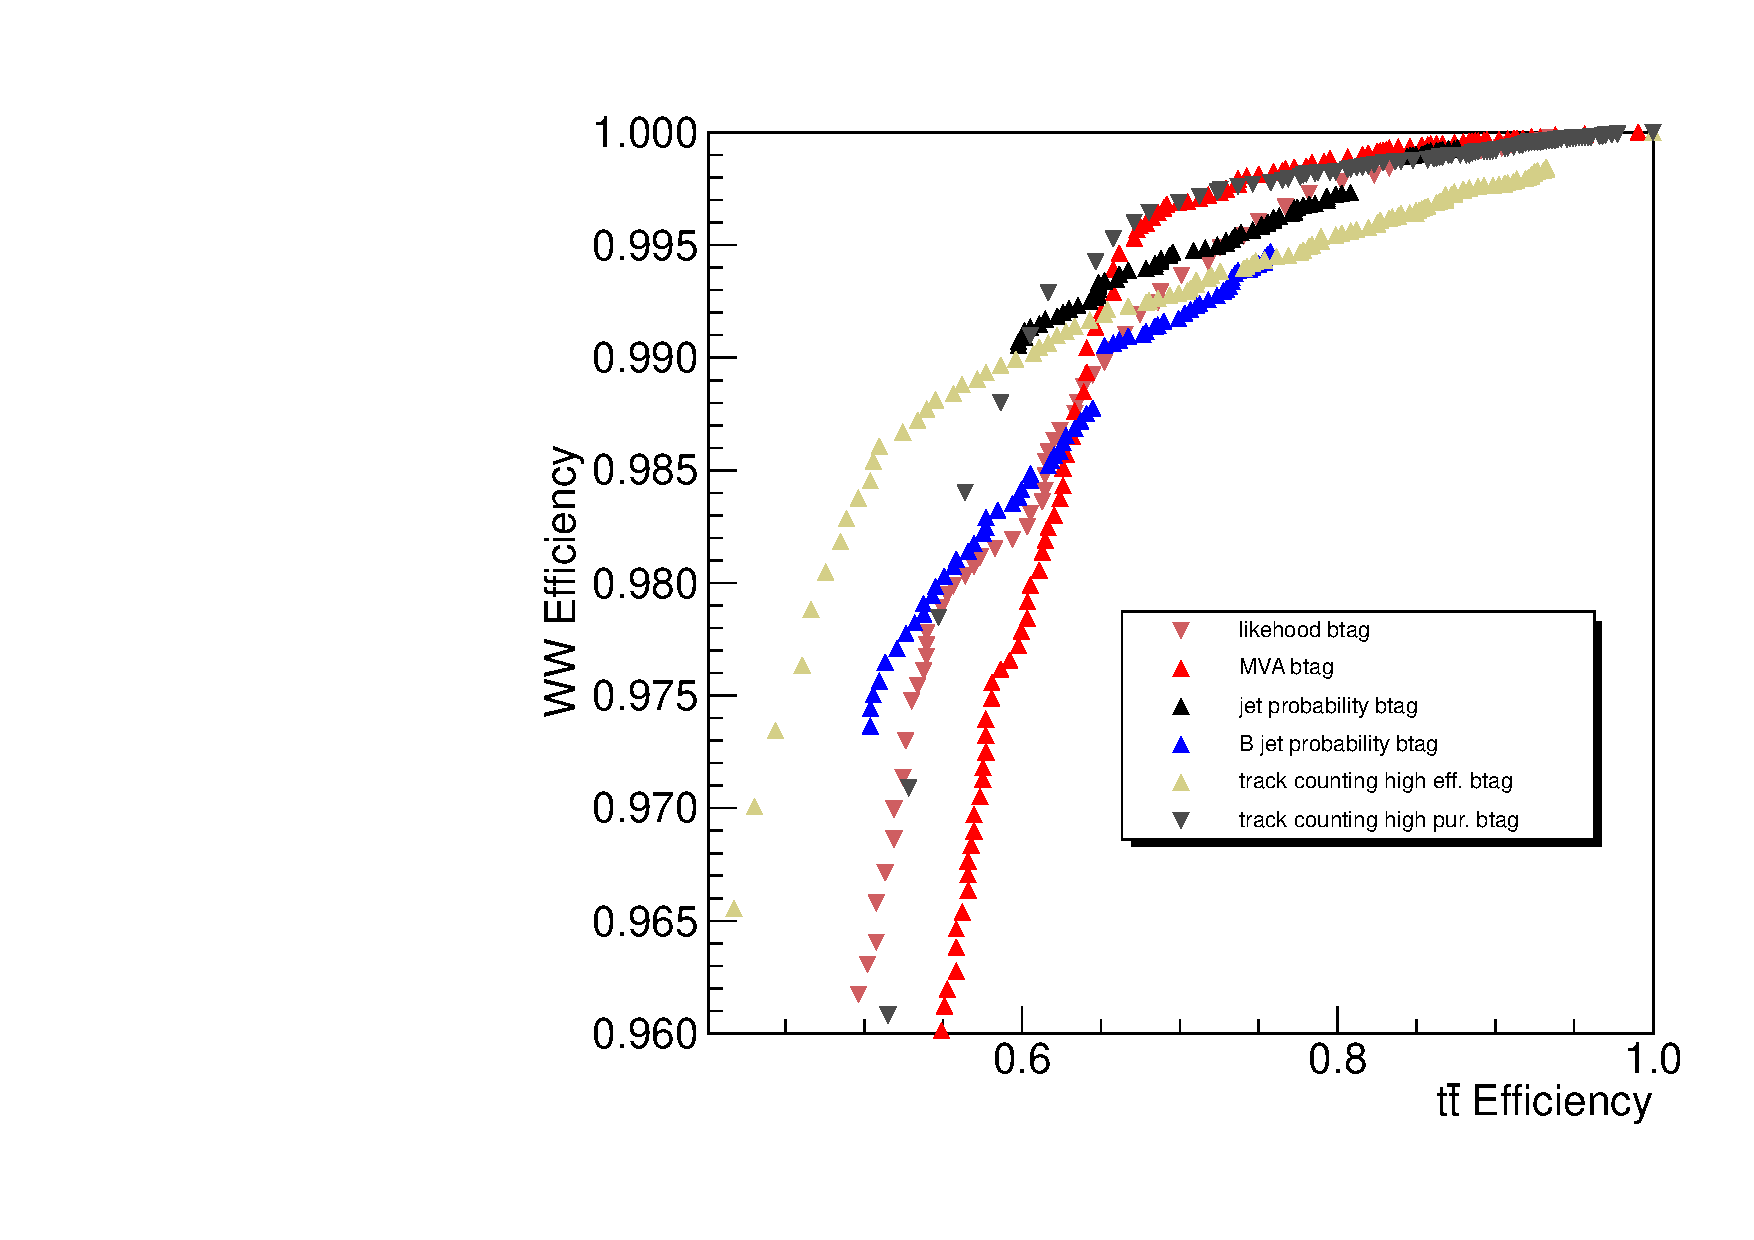
\includegraphics[width=0.60\textwidth]{figures/eff_btag_tt_ww.pdf}
\caption{$\WW$ signal efficiency versus $\ttbar$ efficiency in events with no
reconstructed jets for different standard b-tagging algorithms.}
\label{fig:eff_btag_tt_ww}
\end{center}
\end{figure}
